%~ \subsection{Model and Implementation}
%~ I will desribe the model in this section in a bottom-up fashion.
%~ First describing all parts and then connecting them.

%~ \subsubsection{Graphs}
    %~ A graph is a set of nodes \(V\) and edges \(E\).
\subsection{Gabriel- and Relative Neighborhood Graph}
\label{ssec:graphtypes}
    A graph \(G(V,E)\) is a set of nodes \(V\) and edges \(E\).\\
    All here mentioned graph types are \emph{proximity graphs}. They are
    connecting nodes which are by some metric near to each other.
    Hence they are suited to generalize problems defined on regular
    lattices with nearest neighbor relationships, like the Ising model
    which will be described in more detail in section
    \ref{ssec:isingmodel}.
    In this thesis the distance is always determined by the Euclidian
    metric in two dimensions, though in principle every metric in any
    dimension can be used.\\

    The Gabriel graph \cite{Gabriel1969} is a subgraph of the
    Delaunay triangulation. Two nodes \(i\) and \(j\) with distance
    \(d_{ij}\) are connected with an edge, if a circle with it's
    center on the middlepoint between \(i\) and \(j\) and radius
    \(r = \frac d 2\) contains no other nodes. This area will be
    called \emph{lune} in the following. See also Figure
    \ref{fig:lunes}\subref{sfig:lunes:def}.\\
    The Relative Neighborhood graph \cite{Toussaint1980} is a
    subgraph of the Gabriel graph. Two nodes \(i\) and \(j\) with
    distance \(d_{ij}\) are connected, if no other node is in the
    \emph{lune}. The lune is defined as the intersection of two
    circles with radius \(r = d\) and centers on \(i\) and \(j\).
    See also Figure \ref{fig:lunes}\subref{sfig:lunes:def}.
    \begin{figure}[htbp]
        \centering
        \subfigure[Definition of the lunes][]{
            \label{sfig:lunes:def}
            \tikzset{
    hatch distance/.store in=\hatchdistance,
    hatch distance=10pt,
    hatch thickness/.store in=\hatchthickness,
    hatch thickness=2pt
}

\makeatletter
\pgfdeclarepatternformonly[\hatchdistance,\hatchthickness]{flexible hatch no}
{\pgfqpoint{0pt}{0pt}}
{\pgfqpoint{\hatchdistance}{\hatchdistance}}
{\pgfpoint{\hatchdistance-1pt}{\hatchdistance-1pt}}%
{
    \pgfsetcolor{\tikz@pattern@color}
    \pgfsetlinewidth{\hatchthickness}
    \pgfpathmoveto{\pgfqpoint{0pt}{0pt}}
    \pgfpathlineto{\pgfqpoint{\hatchdistance}{\hatchdistance}}
    \pgfusepath{stroke}
}
\makeatletter
\pgfdeclarepatternformonly[\hatchdistance,\hatchthickness]{flexible hatch nw}
{\pgfqpoint{0pt}{0pt}}
{\pgfqpoint{\hatchdistance}{\hatchdistance}}
{\pgfpoint{\hatchdistance-1pt}{\hatchdistance-1pt}}%
{
    \pgfsetcolor{\tikz@pattern@color}
    \pgfsetlinewidth{\hatchthickness}
    \pgfpathmoveto{\pgfqpoint{0pt}{\hatchdistance}}
    \pgfpathlineto{\pgfqpoint{\hatchdistance}{0pt}}
    \pgfusepath{stroke}
}

\begin{tikzpicture}
    \clip (-2,2.25) rectangle (2,-1.75);

    \begin{scope}
        \clip (-1, 0.5) circle(2.06155281281);
        %~ \fill[fill=blue!20] (1, 0) circle(2.06155281281);
        %~ \draw[pattern=north west lines] (1, 0) circle(2.06155281281);
        \draw[pattern=flexible hatch no,hatch distance=10pt,hatch thickness=0.7pt] (1, 0) circle(2.06155281281);
    \end{scope}

    %~ \fill[fill=white] (0, 0.25) circle(1.0307764064);
    %~ \draw[pattern=north east lines] (0, 0.25) circle(1.0307764064);
    \draw[pattern=flexible hatch nw,hatch distance=10pt,hatch thickness=0.7pt] (0, 0.25) circle(1.0307764064);
    \draw[thick] (0, 0.25) circle(1.0307764064);

    \draw[thick] (-1, 0.5) circle(2.06155281281);
    \fill (-1, 0.5) circle(0.1);
    \draw[thick] (1, 0) circle(2.06155281281);
    \fill (1, 0) circle(0.1);
    \draw[thick] (1, 0) -- (-1, 0.5);
\end{tikzpicture}

        }
        \subfigure[Relative Neighborhood graph example][]{
            \label{sfig:lunes:rng}
            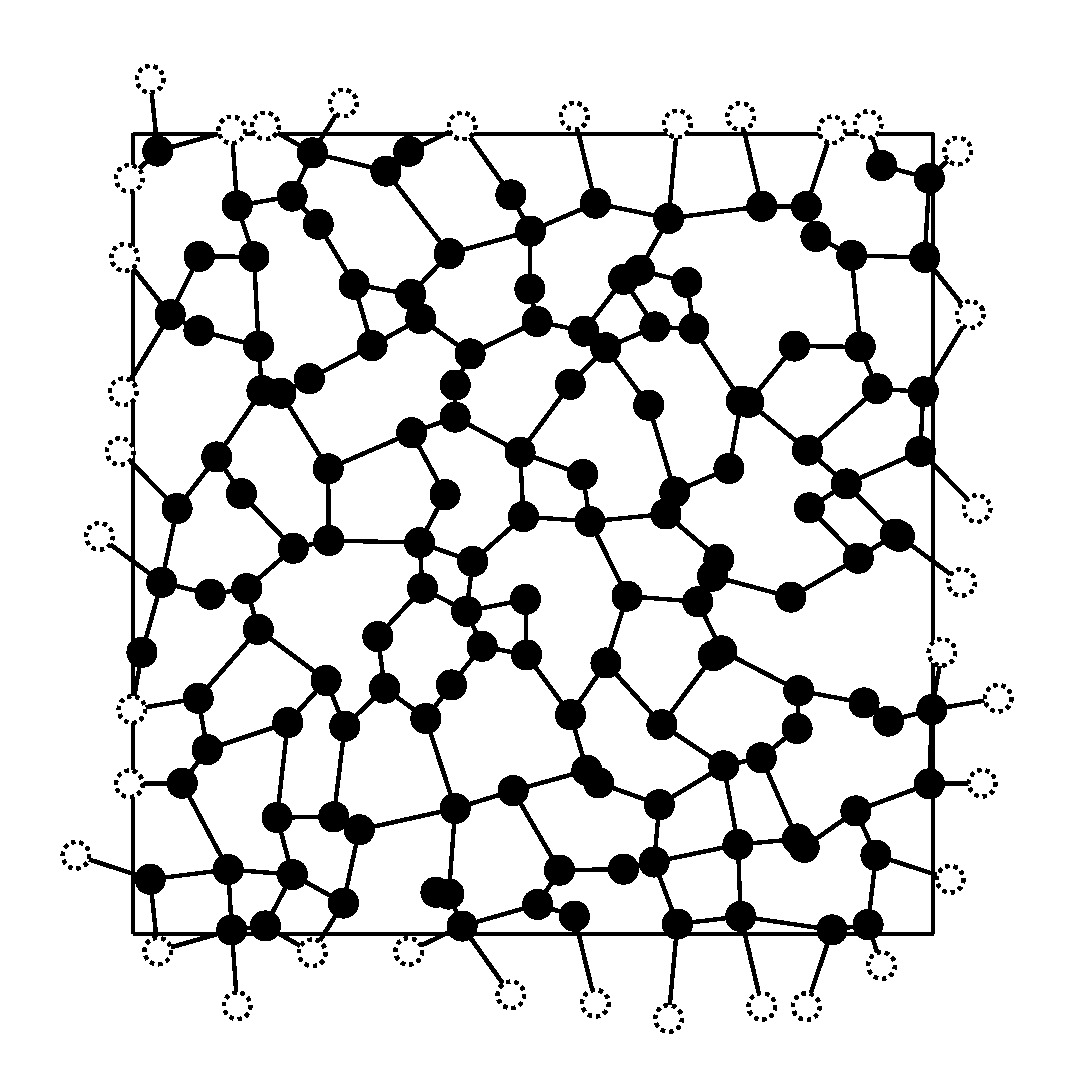
\includegraphics[width=0.3\textwidth]{images/RNG/L12S03.pdf}
        }
        \subfigure[Gabriel graph example][]{
            \label{sfig:lunes:gg}
            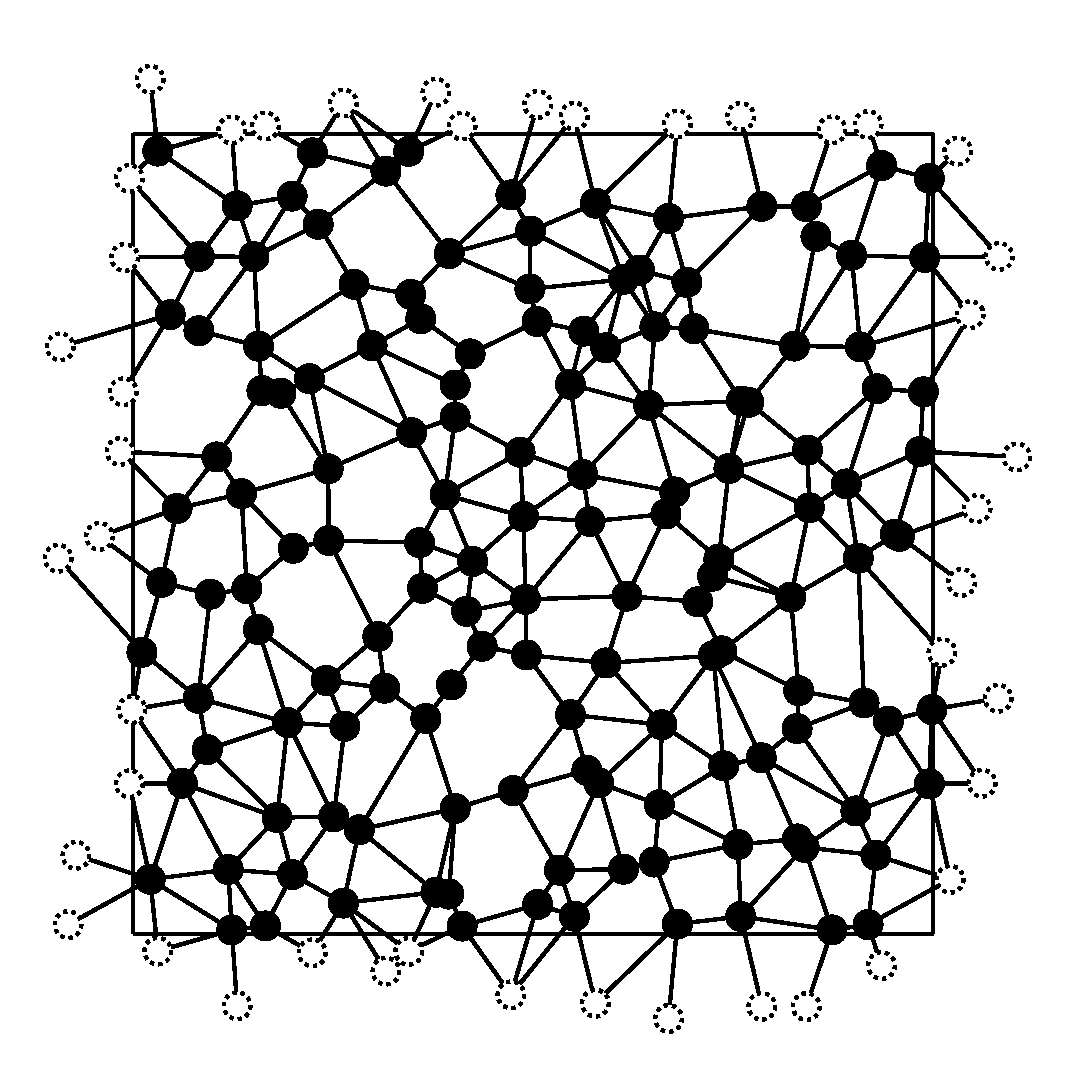
\includegraphics[width=0.3\textwidth]{images/GG/L12S03.pdf}
        }
        \caption[Gabriel - and Relative Neighborhood Graph]
        {
            \subref{sfig:lunes:def} Lunes of Relative Neighborhood
                Graph (hatched region) and
                Gabriel Graph (cross hatched region)
            \subref{sfig:lunes:rng} Example of a Relative
                Neighborhood Graph on periodic boundary conditions.
                Periodic nodes are dashed.
            \subref{sfig:lunes:gg} Example of a Gabriel Graph on
                periodic boundary conditions. Periodic nodes are
                dashed.
        }
        \label{fig:lunes}
    \end{figure}\\
    To construct these graphs the simple way is to test for each
    pair of nodes one has to check for every other node if it lies in
    the lune of the pair. That is of complexity \(O (N^3)\), because
    there are \(N(N-1)\) pairs and for each \(N-2\) nodes to test. So
    the product is of order \(O(N^3)\)\\
    To reduce the complexity one can first create a Delaunay
    Triangulation in complexity \(O (N \log N)\)
    \cite{Leach1992} and test the criterion for each edge, because
    the Delaunay triangulation is a supergraph of both. But the
    implementation of a Delaunay triangulation algorithm is not trivial
    and the generation of the graphs is not time critical in the scope
    of this bachelor thesis.\\
    So a tradeoff is to use basicly the simple method but only test
    the criterion for nodes which are near to the lune and abort if
    one node inside the lune is found. To determine which nodes are
    near the lune one can subdivide the area in \emph{cells} and save
    for each cell a list with nodes lying inside it like presented in
    \cite{RNGCell}.
    Now it is just neccessary to test the nodes in the cells which
    resemble a rectangular bounding box of the lune. Most pairs will be
    far away from each other and the cells in the middle of the bounding
    box are completely inside the lune so that only one node has to be
    tested to discard an edge between them. Connected nodes are near to
    each other so that only very few cells have to be tested.\\
    Indeed this method reduced the time needed to construct a Relative
    Neighborhood graph with \(N=32^2\) and \(N=64^2\) by a factor of
    over \(15\) respectivly \(40\). Though the complexity is still of
    order \(O(N^2)\) in the best case, because for every pair at least
    one check has to be performed.

\subsection{The Disordered Ising Model}
\label{ssec:isingmodel}
    The examined model is a modified 2D Ising model where the \(N=L^2\)
    sites are displaced nodes of a square lattice of edge length \(L\)
    with periodic boundary conditions. The displacement is randomly gauss
    distributed with the standard deviation \(\sigma\). This \(\sigma\)
    is also called \emph{disorder paramter} in the following.
    \begin{equation}
        \hat{H} = \sum_{\avg{i,j}}J_{ij}s_{i}s_{j} - H \sum_i s_i
        \label{eq:hamiltonian}
    \end{equation}
    Equation \eqref{eq:hamiltonian} is the hamiltonian of the Ising model.
    The magnetic field \(H=0\) in the scope of this thesis.
    \(\avg{i,j}\) refers to nodes \(i\) and \(j\) connected by an edge \(E_{ij}\).
    The edges are constructed according to one of the two the in section
    \ref{ssec:graphtypes} defined rules. So that the lattice represents
    a proximity graph. Each node \(i\) has a spin \(s_i = \pm 1\). Each
    edge \(E_{ij}\) has a weight \(J_{ij} = \exp (\alpha (1-d_{ij}))\).
    \(d_{ij}\) is the Euclidian distance between the nodes \(i\) and
    \(j\) and \(\alpha = 0.5\). \(J\) is called \emph{coupling constant}.
    This is definition is inspired by \cite{Lima2000}.\\
    For \(\sigma = 0\) this is the standard Ising model with \(J = 1\),
    for which exists an analytical solution \cite{Onsager1944}.\\

    For evaluation the Monte Carlo simulation is is run till the system
    is equilibrated after \(t_{eq}\) sweeps. Then the simulation continues
    and the magnetisation per site \(m\) and energy per site \(E\)
    are calculated and saved for every \(2\tau\) sweeps. Where \(\tau\)
    denotes the \emph{autocorrelation time} (see also \ref{ssec:eqtime}).
    For every observable \(O\) the expected value \(\avg{O}\) is determined
    as the mean of \(10000\) measurements for \(L=16,32\) or \(5000\) for
    \(L=64,128\). The expected values \(\avg{O}\) for \(100\) different
    random proximity graphs with the same disorder paramter \(\sigma\)
    are then averaged to \(\overline{\avg{O}}\). The errors are estimated
    by bootstrapping.

\subsection{Critical Temperature $T_c$ and Critical Exponents}
\label{ssec:finitesize}
    The aim of this thesis is to find the critical temperature \(T_c\)
    of the disordered Ising model in dependence of the disorder parameter
    \(\sigma\). At \(T_c\) the mean absolute magnetisation \(\avg{|m|}\) of
    the system will jump and the susceptibility
    \(\chi = \frac{N}{T}\brac{\avg{m^2}-\avg{m}^2}\)
    will diverge. In fig. \ref{fig:smeared_out}\subref{sfig:smeared_out:meanM}
    it is easy to see that the jump occurs at lower temperatures \(T\) for higher
    disorder parameters \(\sigma\) (here with a Relative Neighborhood graph).
    \begin{figure}[htbp]
        \centering
        \subfigure[Dependence of the phase transition on $\sigma$][]
        {
            \label{sfig:smeared_out:meanM_L}
            \includegraphics[width=0.45\textwidth]{plots/Mean_M_L_128}
        }
        \subfigure[Example for finite size effects][]
        {
            \label{sfig:smeared_out:meanM}
            \includegraphics[width=0.45\textwidth]{plots/meanM}
        }
        \caption[Phase Transition and Finite Size Effects]
        {
            \subref{sfig:smeared_out:meanM_L}: Effects of the disorder
            parameter $\sigma$ on the phase transition
            for an underlying Relative Neighborhood graph with $L=128$.\\
            \subref{sfig:smeared_out:meanM}: Effects of different system
            sizes at \(\sigma = 0\). Dotted lines are guides to the eye.
        }
        \label{fig:smeared_out}
    \end{figure}\\
    But in the shown plots there occurs no real jump, but a continuous
    decline. The jump is only present in infinite systems, hence every
    computer simulation will show some \emph{finte size effects}.
    These finite size effects cause a "smearing out" of the phase
    trasition. This is stronger for smaller system sizes, as is visible
    in fig. \ref{fig:smeared_out}\subref{sfig:smeared_out:meanM}. Clearly
    the \(L=16\) curve is much less steep than the \(L=128\) curve.\\
    Despite of this one can obtain \(T_c\) by finite size scaling
    methods \cite[S. ??]{NewmanBarkema1999} which also yield the critical
    exponents.
    Studies on random lattices with variing coupling constants \(J\)
    \cite{Lima2000} and without \cite{Janke1994} suggest, that the
    critical exponents should not be influenced by the disorder paramter
    \(\sigma\). So they will be used for consistency cross checking and
    comparision with the known exact values \cite[S. 59]{Pelissetto2002}.\\
    It is known, that for large \(L\) near the critical temperature the
    equations \eqref{eq:fsscaling:m}, \eqref{eq:fsscaling:chi} and
    \eqref{eq:fsscaling:g} apply \cite[p. 145f]{Katzgraber2011}.
    \begin{align}
        \label{eq:fsscaling:m}
        \avg{m_L} &= L^\frac{\beta}{\nu} \tilde{M}\brac{L^\frac{1}{\nu}\brac{T-T_c}}\\
        \label{eq:fsscaling:chi}
        \chi_L    &= L^\frac{\gamma}{\nu} \tilde{C}\brac{L^\frac{1}{\nu}\brac{T-T_c}}\\
        \label{eq:fsscaling:g}
        g         &\propto \tilde{G}\brac{L^\frac{1}{\nu}\brac{T-T_c}}
    \end{align}
    Where \(g = 3-\frac{\avg{m^4}}{2\avg{m^2}^2}\) \cite{Binder1981} is
    the Binder cumulant and \(\tilde{M}, \tilde{C}\) and \(\tilde{G}\)
    are unkown scaling functions. To find the exponents
    \(\beta, \gamma, \nu\) and the critical temperature \(T_c\), one
    varies them until the measured values of the observables collapse on
    one curve. Like the obersables from fig. \ref{fig:gettingCrit}\subref{sfig:gettingCrit:binder_fit_s_0}
    collapse in fig. \ref{fig:gettingCrit}\subref{sfig:gettingCrit:collapse_s_0}.
    Note that \(L=16\) is not used for the collapse, because it is a
    rather small value such that eq. \eqref{eq:fsscaling:m}-\eqref{eq:fsscaling:g}
    do not apply very good.\\
    To accomplish the collapse in an semi-automatic and reproduceable
    way with an error estimate, the programm
    \texttt{autoscale.py} \cite{autoscale2009} is used.
    \begin{figure}[htbp]
        \centering
        \subfigure[Example of a Binder cumulant to determine the critical temperature][]{
            \label{sfig:gettingCrit:binder_fit_s_0}
            \includegraphics[width=0.47\textwidth]{plots/binder_fit_s_0}
        }
        \subfigure[Example of a datacollapse to determine critical exponents][]{
            \label{sfig:gettingCrit:collapse_s_0}
            \includegraphics[width=0.47\textwidth]{plots/collapse_s_0}
        }
        \caption[Examples of determining critical temperature and exponents]
        {
            The Binder cumulant \(g\) of an square lattice Ising model
            (\(\sigma=0\))\\
            \subref{sfig:gettingCrit:binder_fit_s_0} interpolated
                with cubic splines (the errorbars are too small to see)\\
            \subref{sfig:gettingCrit:collapse_s_0} collapsed by finite
                size scaling
        }
        \label{fig:gettingCrit}
    \end{figure}\\
    Though if one is just interested in the critical Temperature, an
    easier approach is to find the intersections of the Binder cumulants
    \(g\) of different system sizes \(L\) because they are intersecting
    at \(T_c\) \cite{Binder1981}.
    Therefore a cubic spline interpolation\footnote{created using the \texttt{scipy.interpolate} tools \cite{scipy2001}}
    is calculated for the measured points.
    As an example take fig. \ref{fig:gettingCrit}\subref{sfig:gettingCrit:binder_fit_s_0}.
    Here such interpolations are plotted for \(\sigma=0\) and are
    intersecting at \(\approx 2.27\).
    To determine \(T_c\) the intersections\footnote{found using the \texttt{scipy.optimize} tools \cite{scipy2001}}
    are averaged and the standard error is calculated. In this case one
    gets \(T_c = 2.2689(2)\), which is in good agreement with the
    exact solution from eq. \eqref{eq:exactTc} \cite{Onsager1944}.
    \begin{equation}
        T_c = 2J/\ln(1+\sqrt 2) = 2.2691...
        \label{eq:exactTc}
    \end{equation}

% Erwahnen, dass T_c Graph so aussieht, wie degree graph
% mit theo ergebnissen von Honeycomb \cite{Wannier1945} vergleichen (fur deg = 3)
% cosh(2L_c)=2 mit L_c = J/2kT_c -> T_c \approx 1.52
